\section{Tests}
\label{sec:Tests}

For this TP we are also required to create some unit tests to make sure that the calculation are carried out properly and that there are no errors in the code. 
The test are written in JAVA and run directly in the SimTG / Eclipse environment.
We tested the models first individually and then combined with the whole CSS. 
Finally, we tested the AOCS controller together with the CSS model.

An example of the output of a test for the Cell model can be seen below in \autoref{fig:test_example} the JAVA source code for a test file can be seen in \autoref{sec:test_example}.

\begin{figure}[H]
    \centering
    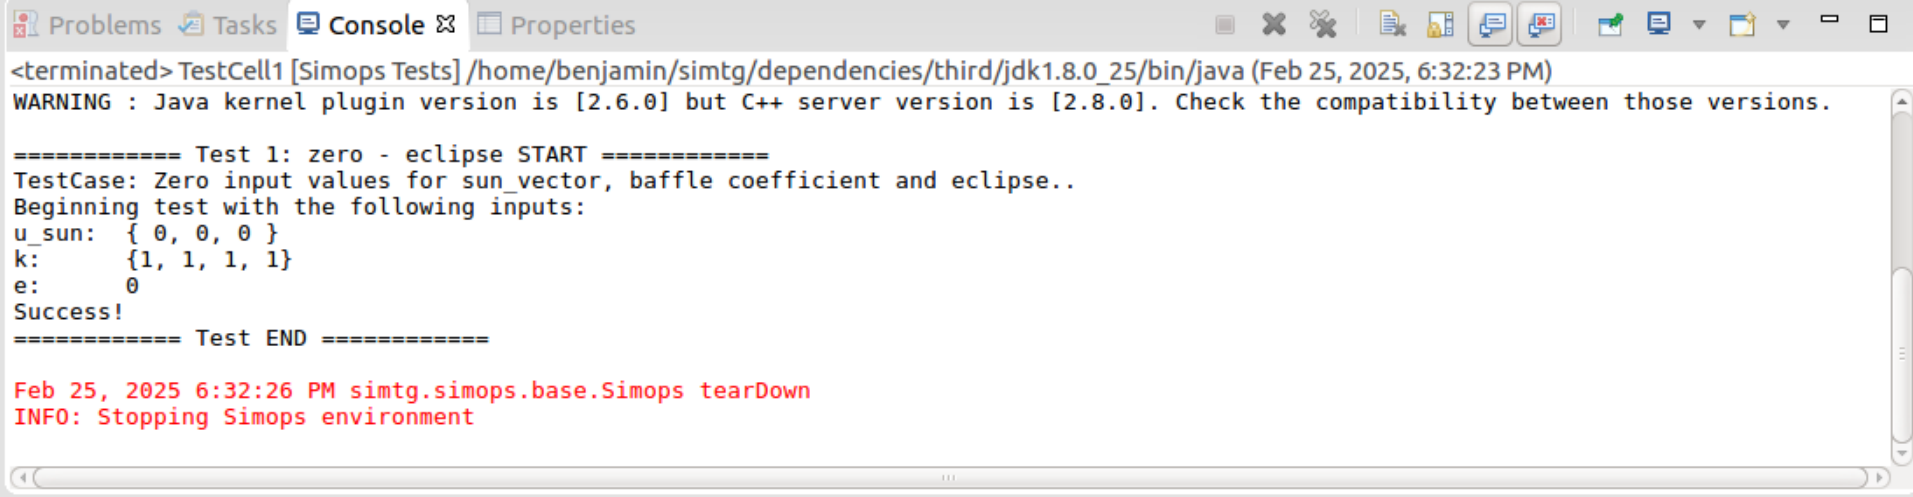
\includegraphics[width=1\linewidth]{doc//Graphics/test_example.png}
    \caption{Example output of Cell test when sun vector is 0 and the satellite is in eclipse.}
    \label{fig:test_example}
\end{figure}

An example of the output of a test for the CSS model can be seen below in \autoref{fig:test_example_CSS}.

\begin{figure}[H]
    \centering
    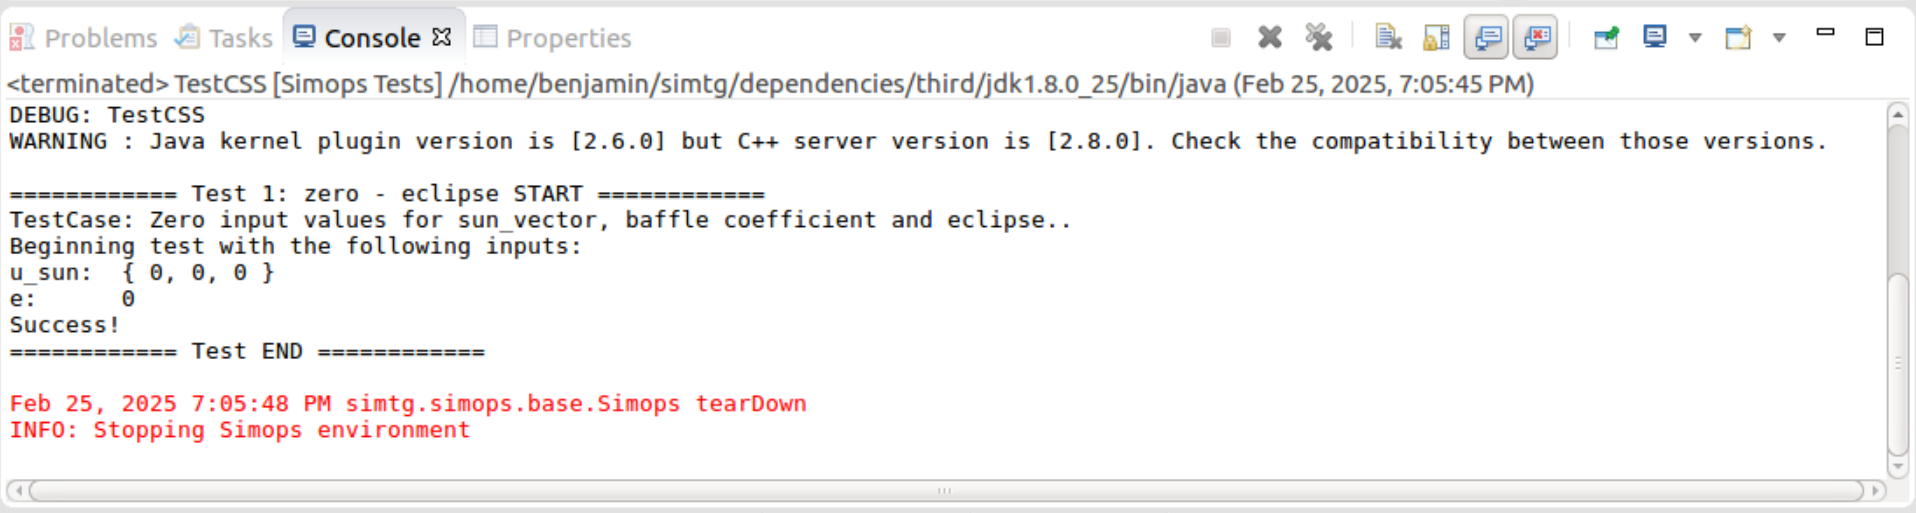
\includegraphics[width=1\linewidth]{doc//Graphics/test_example_CSS.png}
    \caption{Example output of CSS test when sun vector is 0 and the satellite is in eclipse}
    \label{fig:test_example_CSS}
\end{figure}


For the sake of readability of the report, we won't include all of the test files nor the output of them here, but will instead list the test cases and the results for them in the table below.


\newpage
\subsection{Testing Table}
\begin{table}[H]
\centering
    \begin{tabularx}{\textwidth} {
    | >{\hsize=0.35\hsize}X      % Test No.
    | >{\hsize=1.55\hsize}X      % Description
    | >{\hsize=0.8\hsize}X      % Expected Output
    | >{\hsize=0.3\hsize}X      % Status
    |}
    \hline
    \textbf{Model} & \textbf{Description} & \textbf{Expected output} & \textbf{Status} \\ \hline\hline
    
    Cell & Zero values for $\Vec{u}_{sun}$, k and e & $I_{cell} = 0.0$ & \PASS \\ \hline
    Cell & Normal values for $\Vec{u}_{sun}$, k and e=0. & $I_{cell} = 0.0 $ & \PASS \\ \hline
    Cell & Normal values for $\Vec{u}_{sun}$ and k=1 and e=0. & $I_{cell} = 0.0 $ & \PASS \\ \hline
    Cell & Normal values for $\Vec{u}_{sun}$, k and e=1. Test that output is not zero. & $I_{cell}$ not 0 & \PASS \\ \hline
    Cell & Specific values for $\Vec{u}_{sun} = (1, 0, 0)$, k and e=1. Test that output matches mathematically to MatLab script. & $I_{cell}$ = 0.010825224571338 & \PASS  \\ \hline
    Cell & Specific values for $\Vec{u}_{sun} = (0, 1, 1)$, k and e=1. Test that output matches mathematically to MatLab script. & $I_{cell}$ = 0.028742661027327 & \PASS \\ \hline
    CSS & Zero values for $\Vec{u}_{sun}$ and e & All $I_{cell}$ components = 0 & \PASS \\ \hline 
    CSS & Real values for $\Vec{u}_{sun}$, e = 0 & Same as above & \PASS \\ \hline
    CSS & Real values for $\Vec{u}_{sun}$ and e = 1. For some reason gives 0 as output? & All $I_{cell}$ components not 0 &  \FAIL \\ \hline
    Controller (PID) & Converge to 0 with any initial value & After some iterations, angle = 0 &  \PASS \\ \hline
    Satellite & A simple test with the complete model & Non-zero output &  \FAIL \\ \hline
        
    \end{tabularx}
    
\end{table}

\subsection{Testing Controller}
%\TODO{Henkka lisää jotain paskaa tänne}
The complete model of the satellite could not be done in time. Therefore, only the PID-controller is tested on its own. In the complete model, the inputs for the PID-controller are the currents of the sun sensors. To test the PID-controller, the input is set to the output of the controller. The initial angles are random, 100 for y-axis, and 52 for z-axis. On every iteration, the PID-controller calculates a new output, and on the next iteration this output is used as the input.

The outputs are written into a CSV-file and the values are plotted using Python. There are a little over 100 iterations in the testing code. As we can see in the figure, the controller is not acting quite right. The output should be resembling a sinusoidal function that dampens over time towards zero. However, the PID-controller does converge to zero, so the end result is correct.

\begin{figure}[H]
    \centering
    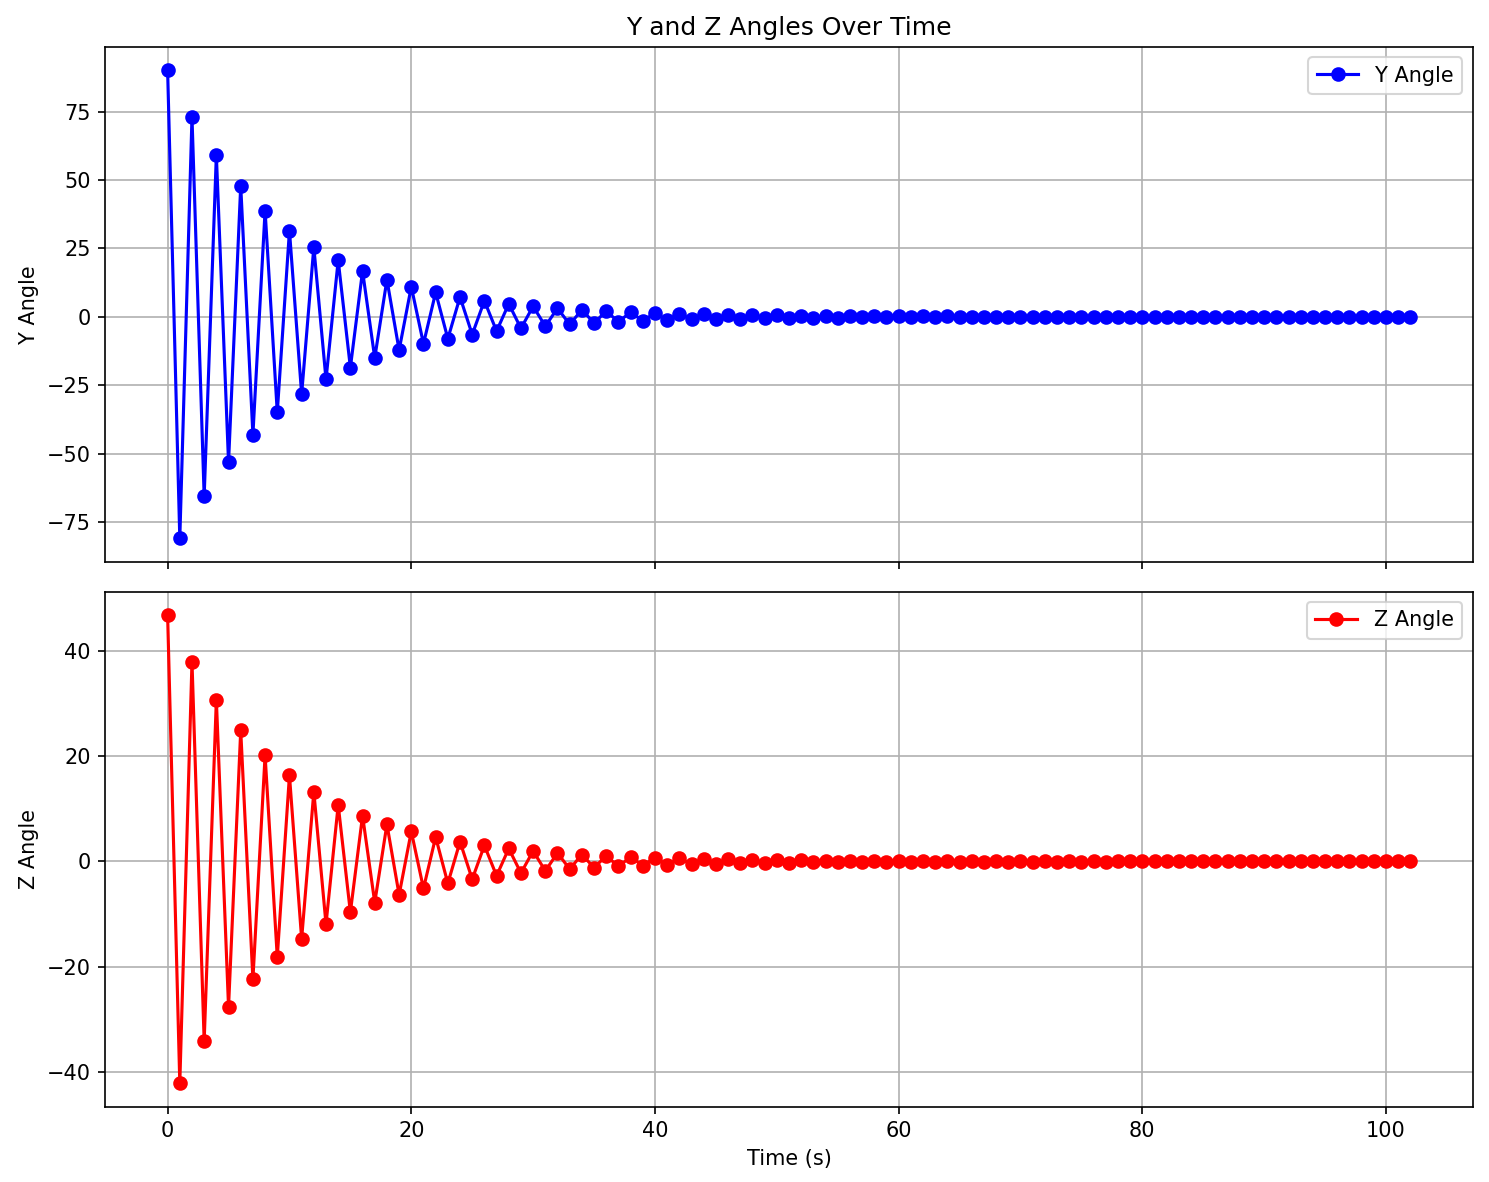
\includegraphics[width=1.0\linewidth]{doc//Graphics/y and z angles.png}
    \caption{The PID converging}
    \label{fig:pid}
\end{figure}

\subsection{Testing Satellite}
Testing the satellite is done by giving it an initial Sun's direction vector, and then in a loop feeding the output back to the input. This feedback loop should iteratively change the satellite's Sun vector into equal with the vector in which the solar arrays are pointed towards. However, we could not get a simple test working (the output is bunch of zeroes) and we were running out of time. Fixing the satellite model would require more testing of the individual models to find out which part is outputting the zeroes.